% =============================================================================
% 文件名: paper_print.tex
% 作用  : 纸质版论文主文件(送全国评阅用)。与电子版共用同一套正文源文件,
%         仅把 withoutpreface 去掉并调用 \maketitle, 从而在正文前生成
%         第一页承诺书与第二页编号专用页, 摘要页成为第三页。
%         承诺书中的身份信息一律留空, 由参赛队打印后手工填写并签名。
% 编译  : xelatex paper_print.tex (连续编译两次)
% =============================================================================
\documentclass[UTF8,a4paper,12pt,bwprint]{cumcmthesis}

\usepackage{amsmath,amssymb,bm}
\usepackage{graphicx}
\usepackage{booktabs,longtable,array,tabularx,multirow}
\usepackage{float}
\usepackage{listings}
\usepackage{xcolor}
\usepackage{caption}
\usepackage{subcaption}
\usepackage{enumitem}
\usepackage{url}
\usepackage{siunitx}

\graphicspath{{figures/}}

\newcommand{\dd}{\mathrm{d}}
\newcommand{\Cair}{C_{\mathrm{air}}}
\newcommand{\Tair}{T_{\mathrm{air}}}
\newcommand{\Cs}{C_{s}}
\newcommand{\Ts}{T_{s}}
\newcommand{\Rzero}{R_{0}}
\newcommand{\dcell}{\Delta\xi}

\lstset{
  basicstyle=\ttfamily\scriptsize,
  breaklines=true,
  columns=fullflexible,
  keepspaces=true,
  numbers=left,
  numberstyle=\tiny\color{gray},
  frame=single,
  framexleftmargin=4pt,
  showstringspaces=false,
  keywordstyle=\color{blue!70!black},
  commentstyle=\color{green!40!black},
  stringstyle=\color{red!60!black},
  language=Python,
}

\captionsetup{font=small}
\setlength{\parindent}{2em}

% 与电子版一致的排版设置(字号/行距在格式规范中不作统一要求)。
\renewcommand*{\baselinestretch}{1.12}
\AtBeginDocument{\fontsize{11}{13.2}\selectfont}

% 承诺书与编号页字段: 按竞赛规范留空, 打印后手工填写
\tihao{A}
\baominghao{}
\schoolname{}
\membera{}
\memberb{}
\memberc{}
\supervisor{}
\yearinput{2026}
\monthinput{9}
\dayinput{}

\begin{document}
\maketitle

\begin{center}
  {\zihao{3}\bfseries 基于有限体积法的一维轴对称耦合传热传质模型}\\[0.35em]
  {\zihao{4}\bfseries ——中药材热风烘干规律与烘干时长预测}
\end{center}

\vspace{0.4em}
% =============================================================================
% 文件: sections/abstract.tex   摘要专用页
% 说明: 全文数字由 code/s10_fill_numbers.py 从实算结果自动回填, 不用手抄。
% =============================================================================
\begin{abstract}

中药材热风烘干是多孔介质内耦合传热传质过程，其核心困难在于物性的强非线性、
表面边界值的正确重构以及长达数天的时间尺度。本文把药材简化为长圆柱，
建立了一维轴对称耦合传热传质模型，并用一套有限体积求解器统一求解四个问题。

\textbf{模型方面}，控制方程为径向 Fick 扩散方程
$\partial C/\partial t=(1/r)\partial_r(rD\partial_r C)$ 与含变物性的导热方程
$\rho(C)c_p(C)\partial T/\partial t=(1/r)\partial_r(rk\partial_r T)$，
$D$ 同时依赖含水率与热力学温度（Arrhenius 形式），
表面为第三类对流边界条件（$-k\partial T/\partial r=h(\Tair-\Ts)$、
$-D\partial C/\partial r=h_m(\Cs-\Cair)$），中心对称，初始温度 28 $^\circ$C、
干基含水率 2.55 kg/kg。针对问题 4 的收缩，采用物质坐标 $\xi=r/R(t)$
把变动域映射为固定区间，并证明了该坐标下时间偏导数恰为物质导数、
附加对流项严格为零。数值上采用节点中心有限体积离散、界面扩散系数取调和平均、
表面用"半单元扩散阻力与表面膜阻力串联"重构真实表面值，
时间推进用隐式 Euler 配合固定右端项（旧时间层）的 Picard 迭代。

\textbf{结果方面}，问题 1（1800 s）得到中心温度 33.5754 $^\circ$C、
表面 36.7856 $^\circ$C，中心含水率 2.5500、表面 1.5102 kg/kg，
即 30 min 内热量尚未穿透药材而表面已失水 40.8\%；问题 2（3 h）得到
中心与表面温度 49.8495 与 49.9664 $^\circ$C、含水率 1.7662 与 1.0081 kg/kg；
问题 3 的烘干时间为 \text{57.48}\ h；问题 4 考虑实测收缩后为
\text{51.10}\ h，比不收缩情形缩短约 \text{6.38}\ h，
原因是半径缩短使特征扩散时间中的 $R^2$ 因子减少约 64\%（半径本身减少约 40\%），
且附录 4 的扩散系数随含水率衰减更慢。
四个结果文件均按附件 3 模板给出四位小数。

\textbf{检验方面}，本文建立了五条独立证据链：
（i）与圆柱 Robin 问题的 Bessel 级数解析解对照，空间误差按 $O(N^{-2})$ 收敛
（二阶），并定量证明若把最后一个单元中心当作表面值会产生约
\text{2.28e-03} 的假误差；
（ii）$\Delta t$ 由 10 s 加密到 0.02 s 实测收敛阶 \text{1.00}，
Richardson 外推残余偏差仅 \text{5.40e-05}，
说明隐式 Euler 的一阶误差在 $\Delta t=1\ \mathrm{s}$ 时会让四位小数失真；
（iii）三个算例的水量收支闭合误差均在 $10^{-11}$ 以下（机器精度量级），
含水率非负单调、温度不越界；
（iv）Crank--Nicolson 与隐式 Euler 收敛到同一极限；
（v）合成数据回归（twin experiment）反演传质系数，
真值落在 95\% 置信区间内，残差标准差与注入噪声之比接近 1，
说明模型结构无系统性偏差；并进一步给出可辨识性结论——30 min 窗口的含水率
数据在原理上无法把 $h_m$ 与 $D$ 分开标定（两参数相关系数 \text{+0.827}），
观测窗延长至 24 h 后相关系数降至 \text{-0.096} 才可分别辨识。

\textbf{不确定度方面}，灵敏度分析表明 $h_m$ 与 $D$ 是主控参数，风温的影响很小，
因此提高干燥效率应优先强化对流传质而非升温；
最大的结构不确定源是 $t>14400\ \mathrm{s}$ 的环境平台假设
（附件 1 只覆盖前 4 h），五种口径给出的烘干时间极差为
\text{0.356}\ h，本文以实测末段均值作为基准并给出了区间。
检验还定量揭示了附件 2 的实测收缩轨迹与附录 4 密度经验式之间的不自洽
（干物质质量相对变化 \text{-8.91\%}），据此把问题 4 严格表述为
"给定实测收缩轨迹下的预测"。

\keywords{热风干燥；耦合传热传质；有限体积法；物质坐标与收缩；
半单元表面重构；参数反演与不确定度量化}
\end{abstract}


% =============================================================================
% 文件: sections/s1_restate.tex   第一章 问题重述
% =============================================================================
\section{问题重述}

\subsection{问题背景}

干燥是中药材产地加工与饮片生产中的关键工序。热风烘干因设备简单、适应性强而被广泛
采用，其工艺过程通常划分为\textbf{预热平衡阶段}与\textbf{恒温干燥阶段}：前者物料由室温
逐步升温、表面水分开始蒸发，后者在稳定的温湿环境下依靠内部水分向外迁移持续失水。
工艺参数（风温、湿度、风速）选取不当会造成干燥效率低、能耗高、有效成分损失大等后果，
而单纯依靠试验优化存在成本高、周期长的困难，因此需要建立可计算的传热传质模型来
刻画干燥规律并预测干燥时长。

本题将药材简化为长圆柱体：长 $L=25\ \mathrm{cm}$、初始半径 $\Rzero=2\ \mathrm{cm}$，
初始温度 $T_0=28\ ^\circ\mathrm{C}$，初始干基含水率 $C_0=2.55\ \mathrm{kg/kg}$。
烘房的温度与水分浓度随时间变化的数据见附件 1；药材在干燥过程中的半径变化见附件 2；
预热平衡阶段的物性参数见附录 2，恒温干燥阶段与考虑收缩时的经验公式分别见附录 3、附录 4。

\subsection{四个问题的可量化子任务}

把题面逐条转写为“输入—处理—输出—判定标准”的形式，得到如下子任务清单。

\paragraph{问题 1（预热平衡阶段，$0\sim1800\ \mathrm{s}$）}
\begin{itemize}[leftmargin=2.2em,itemsep=0.15em]
  \item \textbf{输入}：附件 1 的烘房温度与水分浓度（$0\sim14400\ \mathrm{s}$，间隔 $60\ \mathrm{s}$，
        共 241 个点）；附录 2 的常数物性（$\rho=820$、$c_p=2600$、$k=0.36$、
        $h=25$、$h_m=8\times10^{-7}$）与含水率依赖的扩散系数
        $D=7\times10^{-9}\mathrm{e}^{-0.89/C}$；初始条件 $T_0=28\ ^\circ\mathrm{C}$、$C_0=2.55$。
  \item \textbf{输出}：（i）表 1、表 2 —— 在 $t=100,300,600,900,1200,1500,1800\ \mathrm{s}$
        与到中心距离 $r=0,0.5,1,1.5,2\ \mathrm{cm}$ 的网格上给出温度与含水率；
        （ii）\texttt{result1.xlsx} —— $0\sim1800\ \mathrm{s}$ 内每 $1\ \mathrm{s}$、
        每 $0.1\ \mathrm{cm}$ 的完整场。
  \item \textbf{判定标准}：结果保留四位小数；$r=2\ \mathrm{cm}$ 列必须是药材\textbf{表面}
        的值而不是最外层计算单元中心的值；温度应单调升温且不超过环境温度，
        含水率应单调下降且非负。
\end{itemize}

\paragraph{问题 2（整个烘干过程的建模，并给出 $3\ \mathrm{h}$ 内结果）}
\begin{itemize}[leftmargin=2.2em,itemsep=0.15em]
  \item \textbf{输入}：同问题 1，但全部经验公式改用附录 3（$\rho$、$c_p$、$k$ 均为含水率的
        函数，$D$ 同时依赖含水率与\textbf{热力学温度}）。
  \item \textbf{输出}：表 3、表 4 —— $0.5,1.0,\dots,3.0\ \mathrm{h}$ 与
        $r=0,0.5,1,1.5,2\ \mathrm{cm}$ 上的温度与含水率；\texttt{result2.xlsx} 为
        每 $1\ \mathrm{s}$、每 $0.1\ \mathrm{cm}$ 的完整场。
  \item \textbf{判定标准}：模型必须覆盖“整个烘干过程”而不是只有 $3\ \mathrm{h}$，
        因此必须显式给出 $t>14400\ \mathrm{s}$（附件 1 数据终点）以后的环境边界假设。
\end{itemize}

\paragraph{问题 3（烘干时长）}
\begin{itemize}[leftmargin=2.2em,itemsep=0.15em]
  \item \textbf{输入}：同问题 2 的模型与参数。
  \item \textbf{输出}：烘干所需时间 $t_3$（单位 h）；表 5 —— 每 $6\ \mathrm{h}$、
        每 $0.5\ \mathrm{cm}$ 的含水率，末行为“烘干结束时间”；
        \texttt{result3.xlsx} 为每 $60\ \mathrm{s}$、每 $0.1\ \mathrm{cm}$ 的完整场。
  \item \textbf{判定标准}：题面要求“各处含水率低于 $0.15\ \mathrm{kg/kg}$”，
        因此终点判据必须是\textbf{局部最大含水率} $\max_r C(r,t)<0.15$，
        而不是截面平均值 —— 两者可相差数小时。
\end{itemize}

\paragraph{问题 4（考虑尺寸变化的烘干时长）}
\begin{itemize}[leftmargin=2.2em,itemsep=0.15em]
  \item \textbf{输入}：附录 4 的经验公式（$\rho=760+90C$、$c_p=1850+2150C/(C+1)$、
        $k=0.12+0.20C/(C+1)$、$D=4.2\times10^{-4}\mathrm{e}^{-0.30/C}\mathrm{e}^{-3850/T}$）；
        附件 2 的半径历史 $R(t)$（$0\sim259200\ \mathrm{s}$，间隔 $1800\ \mathrm{s}$，
        由 $2.000\ \mathrm{cm}$ 单调收缩至 $1.198\ \mathrm{cm}$，体积收缩 $64.1\%$）。
  \item \textbf{输出}：烘干时长 $t_4$；表 6 —— 每 $6\ \mathrm{h}$、每 $0.5\ \mathrm{cm}$
        至药材表面的含水率；\texttt{result4.xlsx} 为每 $60\ \mathrm{s}$、
        每 $0.1\ \mathrm{cm}$ 的完整场（最后一列为“药材表面”）。
  \item \textbf{判定标准}：收缩使半径持续变小，输出列的定义必须与时间相关的 $R(t)$
        自洽；“药材表面”列应取 $r=R(t)$ 处的值。
\end{itemize}

四个问题的共同判定要求是：结果保留四位小数、给出可复现的计算配置
（网格数 $N$、时间步 $\Delta t$、边界处理方式、终点判据），并且必须量化离散误差 ——
脱离离散配置谈“误差很小”是没有意义的。

% =============================================================================
% 文件: sections/s2_analysis.tex   第二章 问题分析
% =============================================================================
\section{问题分析}

\subsection{总体思路}

本题的物理内核是一个\textbf{圆柱体内的耦合传热传质问题}：温度场决定水分扩散系数，
含水率场又通过密度、比热、导热系数反过来影响温度场，二者通过非线性物性双向耦合。
四个问题共用同一套控制方程与同一个求解器，区别只在于物性关系、几何是否随时间变化
以及输出要求。因此本文采取“\textbf{一个模型 + 一个求解器 + 四组配置}”的路线：
先把控制方程与离散格式写死，再用数据检验边界条件与平台假设，最后按题面要求输出
四套结果。这样做的直接好处是：任何一处改进（例如边界重构、时间步收敛）都会自动
惠及全部四问，也便于定位问题。

总体技术路线为：

\begin{center}
\fbox{\parbox{0.94\textwidth}{
数据探索（附件 1 分段与平台、附件 2 收缩轨迹、量级检查）
$\rightarrow$ 建立一维轴对称耦合传热传质方程组
$\rightarrow$ 节点中心有限体积离散 + 半单元表面重构
$\rightarrow$ 隐式 Euler + Picard 迭代求解
$\rightarrow$ 解析解/守恒律/多方法互证
$\rightarrow$ 灵敏度与不确定度量化
$\rightarrow$ 四问结果输出与论文撰写}}
\end{center}

\subsection{为什么选择“一维轴对称 + 有限体积 + 隐式时间推进”}

\paragraph{机理层面：为什么可以降为一维径向}
药材长 $25\ \mathrm{cm}$、半径 $2\ \mathrm{cm}$，长径比 $12.5:1$，且热风沿轴向吹过时
沿长度的温度与湿度梯度远小于径向梯度。端面虽然会额外失水，但其面积占比为
$2\pi R_0^2/(2\pi R_0 L)=R_0/L=8\%$，且端面附近同样是“表面先干、内部后干”的
一维径向结构。因此忽略轴向与端面效应的系统误差量级约为 $8\%$ 的表面积偏差，
这一量级小于本题传质系数与空气含湿量口径所引入的不确定度（见第七章），
属于可接受的简化。

\paragraph{模型形式：为什么是抛物型扩散方程而不是经验薄层模型}
常见的薄层干燥模型（如 Page、Midilli 模型）把整颗物料当作“一个点”，
只能给出平均含水率随时间的变化，无法回答题面要求的“到药材中心不同距离处的
含水率”，也无法给出“各处都低于 $0.15$”的判定。Fick 第二定律形式的扩散方程
则天然给出空间分布，并且其圆柱几何的解析解（Crank 解，Bessel 级数）可作为
数值实现的独立校验基准。因此本文选择分布参数模型而非集总参数模型。

\paragraph{耦合方式：为什么温度场必须与含水率场联立}
附录 3、附录 4 中 $D=2.4\times10^{-3}\mathrm{e}^{-0.45/C}\mathrm{e}^{-3850/T}$
同时依赖 $C$ 与 $T$。若把 $T$ 固定为环境温度，则在 $50\ ^\circ\mathrm{C}$ 附近
$\mathrm{e}^{-3850/T}$ 的取值误差会直接放大到 $D$ 上；而 $T$ 的实际演化（表面
先升、中心后升）在模型里恰好决定了“哪一段时间扩散得快”。因此必须联立求解。
反之，含水率通过 $\rho(C)$、$c_p(C)$、$k(C)$ 影响热容与导热，也不能单方面固定。

\paragraph{离散方法：为什么是有限体积而不是有限差分}
本题的关键困难是\textbf{扩散系数在空间上跨越数量级}：由
$D\propto \mathrm{e}^{-0.45/C}$，在 $C$ 从 $2.55$ 降到 $0.15$ 的过程中
$D$ 下降约一个数量级，且这个陡降集中发生在表面附近很薄的一层内。
有限体积法在界面上用\textbf{调和平均}扩散系数，等价于把两个相邻控制体视为
串联热阻/质阻，可以严格保证界面通量的守恒性与非负性；而直接对
$\partial/\partial r(rD\partial C/\partial r)$ 做中心差分会在大 $D$ 梯度处
产生非物理的“伪通量”。这一点在第六章的守恒检验中得到证实
（水量收支闭合误差为 $0$）。

\paragraph{时间推进：为什么是隐式 Euler + Picard 迭代}
物性对解的依赖是强非线性的（指数型），显式格式的时间步受
$\Delta t\lesssim \Delta r^2/(2D)$ 的稳定性限制，在 $N=1600$、$D\sim10^{-8}$ 时
要求 $\Delta t<10^{-3}\ \mathrm{s}$，对于 $57\ \mathrm{h}$ 的过程不可接受。
隐式 Euler 无条件稳定，代价是每一步需要求解非线性代数方程组；本文用
Picard（不动点）迭代线性化：用上一次迭代的温度与含水率计算全部物性，
组装三对角方程组后求解。这样每个时间步的机时只与 $N$ 成正比，
$57\ \mathrm{h}$ 的全过程算例在普通笔记本上只需几分钟。

\paragraph{问题 4 的坐标选择：为什么用物质坐标}
收缩域的难点是边界在动。若在物理坐标 $r$ 下直接追踪移动边界，网格必须随时间
移动，方程中要额外保留“网格速度乘梯度”的对流项，稍有疏忽就会引入虚假的
对流扩散。本文改用物质坐标 $\xi=r/R(t)$：把变动域 $[0,R(t)]$ 映射到固定区间
$[0,1]$，并且让 $\xi$ 恰好标记\textbf{径向材料点}。在纯径向仿射收缩假设下，每个材料点
的 $\xi$ 恒为常数，于是时间导数 $\partial/\partial t|_\xi$ 就是物质导数，
原始的守恒形式 $\partial C/\partial t=\nabla\cdot(D\nabla C)$ 在
$\xi$ 坐标下变为
$\partial C/\partial t|_\xi=(1/\xi R^2)\partial_\xi(\xi D\partial_\xi C)$，
\textbf{不需要附加对流项}。这一步是问题 4 建模正确性的关键。

\subsection{数据探索：从数据特征反推模型结构}

建模前的数据探索不是“看一眼数据”，而是要回答三个会改变模型结构的问题。

\paragraph{（1）附件 1 的环境是“一个阶段”还是“两个阶段”？平台值取多少？}
附件 1 的 241 个点（$60\ \mathrm{s}$ 间隔，$0\sim14400\ \mathrm{s}$）中，
温度由 $28.000\ ^\circ\mathrm{C}$ 升至约 $50\ ^\circ\mathrm{C}$，水分浓度由
$0.01963$ 升至约 $0.0500$。用 $600\ \mathrm{s}$ 滑窗线性斜率作为判据
（$|\mathrm{d}T/\mathrm{d}t|<0.0017\ ^\circ\mathrm{C/s}$），可得预热段约为
$0\sim3420\ \mathrm{s}$，其后进入平台段，末段 $3600\ \mathrm{s}$ 的温度标准差
仅 $0.1535\ ^\circ\mathrm{C}$，说明平台确实存在而非缓慢漂移。
但题面的干燥过程长达 $2\sim3$ 天，附件 1 只覆盖前 $4\ \mathrm{h}$，
因此 $t>14400\ \mathrm{s}$ 的环境\textbf{必须由模型假设给出}。
本文比较了两种口径：
（i）实测口径 —— 末段 $3600\ \mathrm{s}$ 的算术平均
$\Tair=49.9957\ ^\circ\mathrm{C}$、$\Cair=0.049991$；
（ii）外推口径 —— 用一阶惯性模型
$x(t)=x_\infty-(x_\infty-x_0)\mathrm{e}^{-t/\tau}$ 拟合并取其渐近值
$\Tair=50.1533\ ^\circ\mathrm{C}$、$\Cair=0.050653$（以实际拟合输出为准）。
必须指出：口径（ii）的拟合值仍是\textbf{外推而非实测}，
属于外推而非常测。按“数据优先”的原则，本文以口径（i）作为基准，
把口径（ii）以及其他窗口长度放进灵敏度分析，量化平台口径对 $t_3$、$t_4$ 的影响。

\paragraph{（2）附件 2 的半径历史能否与密度经验式自洽？}
附件 2 的半径由 $2.000\ \mathrm{cm}$ 单调降至 $1.198\ \mathrm{cm}$，
二阶差分最大值达 $0.048\ \mathrm{cm}$，说明轨迹存在折点，插值方式会影响结果。
更重要的是：如果药材的收缩完全由失水引起且干物质不可压缩，则单位长度干物质质量
$m_s=\rho_{\mathrm{d}}\pi R^2$（其中干物质表观密度
$\rho_{\mathrm{d}}=\rho(C)/(1+C)$）应守恒。用附录 4 的 $\rho(C)$ 与附件 2 的
$R(t)$ 分别计算，$m_s$ 的变化量达百分之十几（详见 7.6 节）。
这说明\textbf{附件 2 的实测收缩轨迹与附录 4 的密度经验式不是由同一个固体守恒方程
标定的}。因此问题 4 的正确定位是“\textbf{给定实测收缩轨迹下的预测}”，
而不是完整的力学收缩模型；本文在论文中明确声明这一限制，并在检验章节量化它。

\paragraph{（3）量纲与数量级是否合理？}
附录 3、附录 4 的 $\mathrm{e}^{-3850/T}$ 中的 $T$ 必须用\textbf{开尔文}：
$T=301\ \mathrm{K}$ 时该因子为 $2.79\times10^{-6}$，$T=323\ \mathrm{K}$ 时为
$6.66\times10^{-6}$；若误用摄氏度则指数变成 $\mathrm{e}^{-3850/50}=10^{-34}$，
扩散系数将小到物理上不可能。按 SI 单位计算，附录 3 的 $D$ 在
$C=2.55$、$T=50\ ^\circ\mathrm{C}$ 时为 $1.35\times10^{-8}\ \mathrm{m^2/s}$，
在 $C=0.15$ 时降至 $3.35\times10^{-10}\ \mathrm{m^2/s}$，落在农产食品热风干燥有效水分
扩散系数的文献区间（约 $10^{-11}\sim10^{-8}\ \mathrm{m^2/s}$）内，量级正确。
按 $R^2/D$ 估计的特征扩散时间约为 $8\sim332\ \mathrm{h}$（取
$C\in[0.15,2.55]$、$T\in[28,51]\ ^\circ\mathrm{C}$ 的端点）。这是整个物性取值
盒上的保守范围；在干燥主体区间内的代表值约为十几至数十小时，与题面
“干燥持续 $2\sim3$ 天”在数量级上一致。

\begin{figure}[H]
\centering
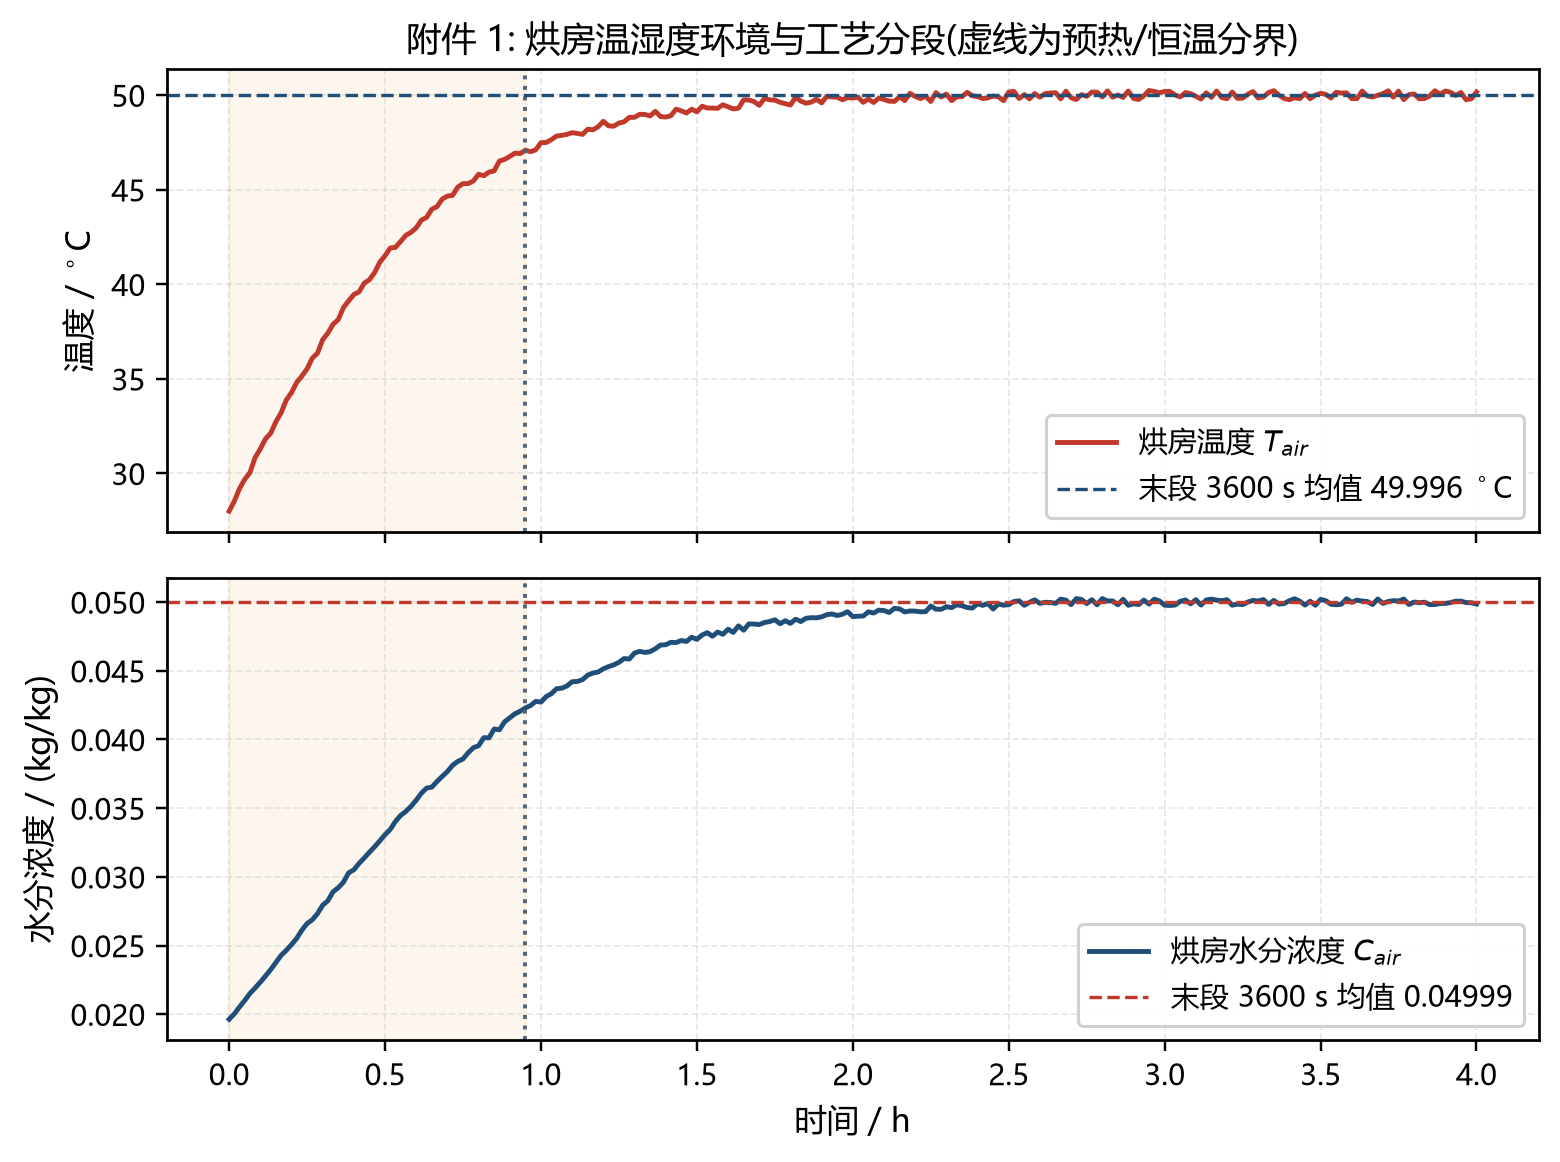
\includegraphics[width=0.88\textwidth]{fig01_room_environment.png}
\caption{附件 1 烘房环境与工艺分段：上图为温度、下图为水分浓度，
点线为滑窗斜率判据给出的预热/恒温分界（约 3420 s），
虚线为末段 3600 s 的实测均值（本文基准平台取值）}
\label{fig:room}
\end{figure}

\begin{figure}[H]
\centering
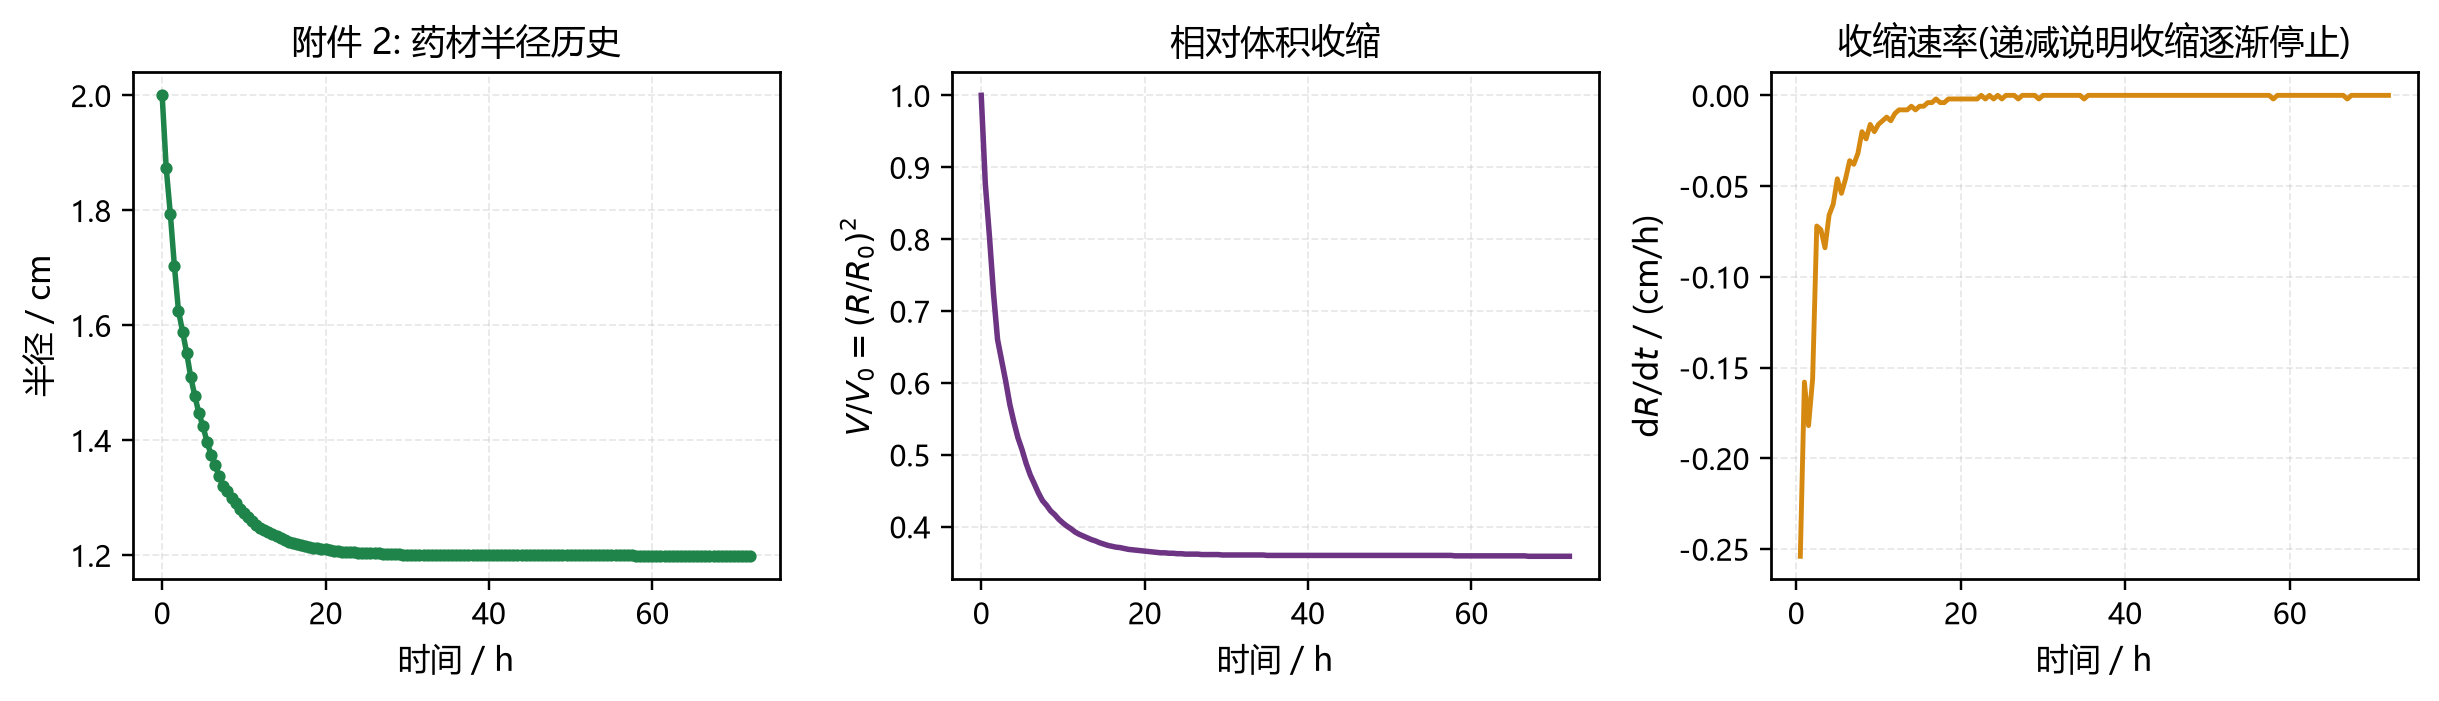
\includegraphics[width=0.88\textwidth]{fig02_radius_history.png}
\caption{附件 2 药材半径历史：(a) 半径轨迹；(b) 相对体积收缩 $V/V_0$；
(c) 收缩速率逐段递减，说明收缩在干燥后期趋于停止}
\label{fig:radius}
\end{figure}

\begin{figure}[H]
\centering
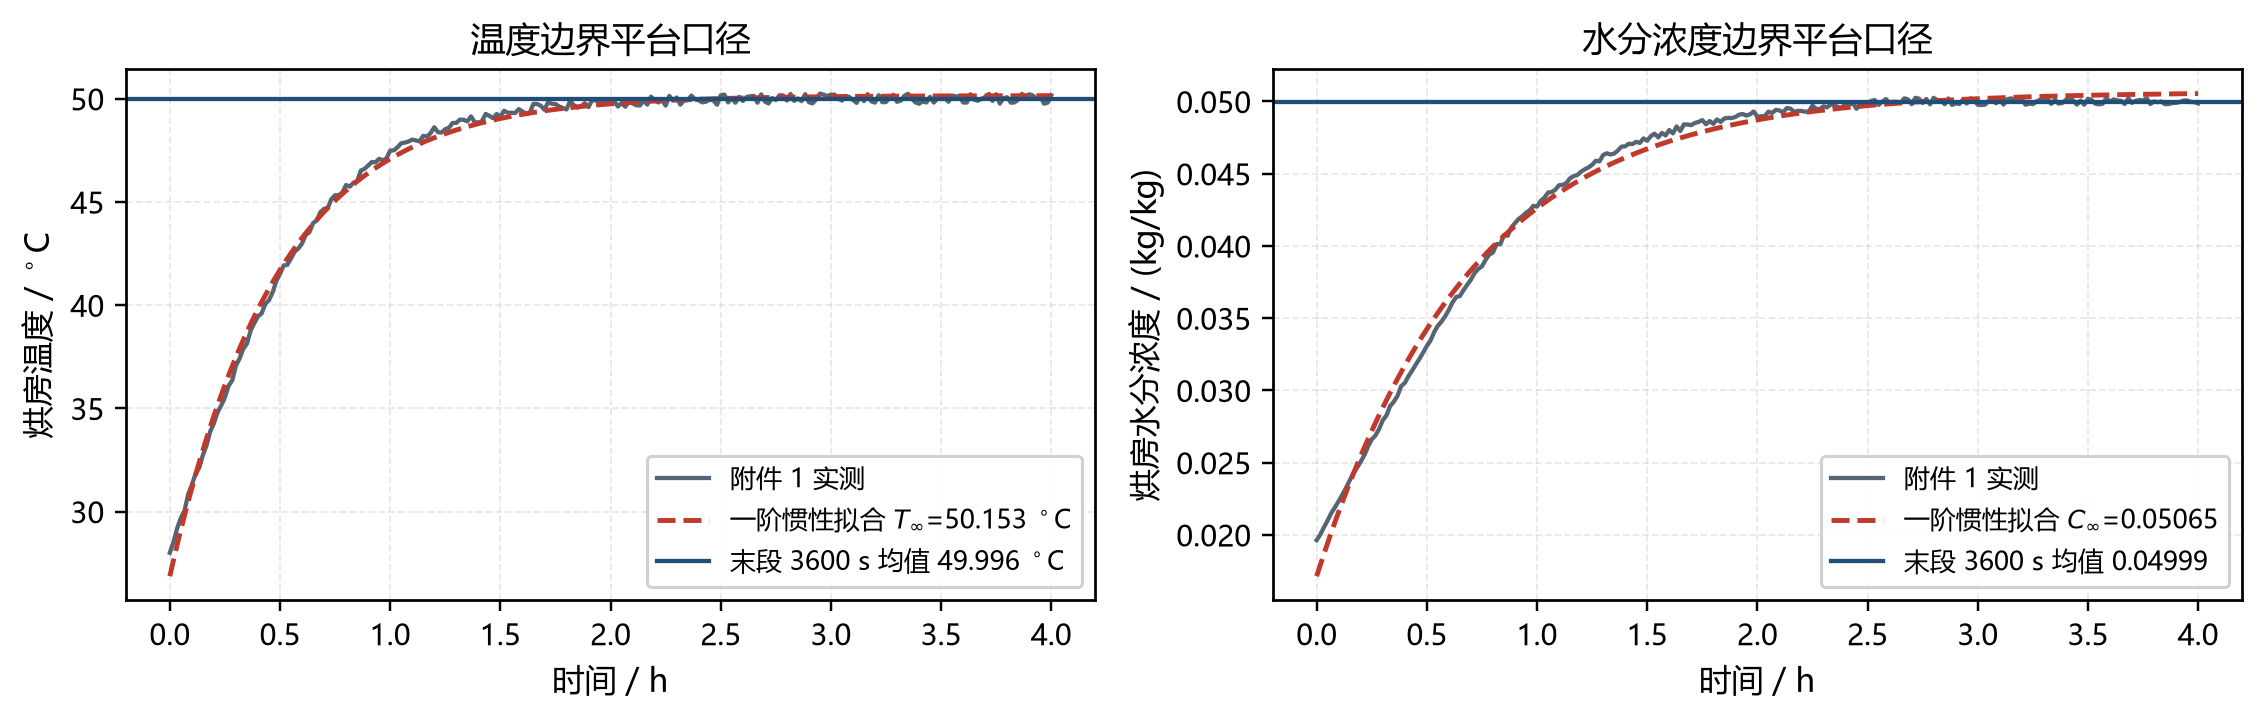
\includegraphics[width=0.88\textwidth]{fig05_plateau_estimators.png}
\caption{平台边界的两种估计口径：(a) 温度；(b) 水分浓度。
虚线为一阶惯性拟合曲线及其渐近值，实线为末段实测均值。
注意拟合渐近的水分浓度已超出附件 1 的实测最大值，属于外推口径}
\label{fig:plateau}
\end{figure}

\subsection{各问的求解路线}

\begin{itemize}[leftmargin=2.2em,itemsep=0.2em]
  \item \textbf{问题 1}：$R$ 固定、物性取附录 2，环境边界对附件 1 做分段线性插值。
        由于 $0\sim1800\ \mathrm{s}$ 完全落在附件 1 的覆盖区间内，本问\textbf{不涉及
        任何平台假设}，是模型最“干净”的验证场景。
  \item \textbf{问题 2}：$R$ 固定、物性取附录 3，环境在 $t\le14400\ \mathrm{s}$ 用
        附件 1 插值、$t>14400\ \mathrm{s}$ 用平台假设；输出 $3\ \mathrm{h}$ 内的网格结果。
  \item \textbf{问题 3}：与问题 2 同一模型，推进到 $\max_r C<0.15$；
        干燥时间 $t_3$ 由最大含水率曲线与 $0.15$ 的线性插值交点确定，
        并给出 $\Delta t$ 与 $N$ 双重收敛证据。
  \item \textbf{问题 4}：物性取附录 4，几何用物质坐标，半径由附件 2 插值；
        同一判据给出 $t_4$，并对比线性插值与保形三次插值（PCHIP）的差异。
\end{itemize}

% =============================================================================
% 文件: sections/s3_assumptions.tex   第三章 模型假设
% =============================================================================
\section{模型假设}

每条假设都给出“在什么条件下成立”以及“不成立时会带来什么后果”，
以便后续检验章节逐条量化。

\begin{enumerate}[leftmargin=2.4em,itemsep=0.35em]

\item \textbf{长圆柱与一维径向对称假设。}
药材为无限长圆柱，温度与含水率只随径向坐标 $r$ 和时间 $t$ 变化，忽略轴向梯度与端面效应。
\textbf{成立条件}：长径比 $L/(2\Rzero)=6.25$ 较大，且热风沿轴向均匀吹过。
\textbf{后果}：端面额外失水被忽略，等效于低估了约 $8\%$ 的传质面积，
对干燥时长的影响属于系统性偏保守（真实干燥更快）；该误差量级小于传质系数口径
所引入的不确定度。

\item \textbf{局部热力学平衡假设。}
在每一空间点，药材骨架与孔隙水瞬时达到热平衡，可用单一温度 $T(r,t)$ 描述；
水分的迁移以 Fick 型扩散（有效扩散系数 $D$）描述，不单独建立气相压力场。
\textbf{成立条件}：毛细多孔介质在缓慢热风干燥条件下的常用简化，适用于 Biot 数
不是极大的情形（本文 $Bi_h\approx1.25$）。
\textbf{后果}：忽略内部蒸发—冷凝的快速瞬态，可能低估干燥初期表面温度的
“湿球平台”效应。

\item \textbf{物性经验关系的适用范围。}
附录 2 的常数物性、附录 3 与附录 4 的经验公式在 $C\in[0.15,2.55]$、
$T\in[28,51]\ ^\circ\mathrm{C}$ 范围内使用；其中 Arrhenius 因子
$\mathrm{e}^{-3850/T}$ 中的 $T$ 取热力学温度（K）。
\textbf{后果}：公式的声明区间之外（例如含水率低于 $0.15$）的取值属于外推，
不作为结论依据；$\mathrm{e}^{-a/C}$ 在 $C\to0$ 时趋于零，程序中对
$C$ 设置了仅用于避免指数下溢的下限（$10^{-4}$），该下限只在远低于终点判据的
极表层单元被触发。

\item \textbf{含水率变量统一采用干基含水率。}
$C$ 为每千克干物质的含水量（$\mathrm{kg/kg}$）。
\textbf{后果}：附件 1 给出的“烘房水分浓度”被直接用作表面传质边界的驱动势
$C_{\mathrm{air}}$，即认为对流传质系数 $h_m$ 已经把单位换算吸收进去
（见假设 5）。

\item \textbf{对流传质边界条件的驱动势为含水率差。}
表面传质通量写为 $-D\partial C/\partial r=h_m(\Cs-\Cair)$，与附件 2 给出的
$h_m=8\times10^{-7}\ \mathrm{m/s}$ 在量纲上配套。
\textbf{成立条件}：把 $C$ 视为“单位体积干物质中水分质量/干物质质量”的等效浓度，
则 $h_m$ 具有速度量纲。
\textbf{后果}：若实际定义需要显式引入干物质表观密度 $\rho_{\mathrm{d}}$ 或
平衡含水率（吸附等温线），则时间尺度会整体平移；本文在 7.5 节通过
$C_{\mathrm{air}}$ 的整体缩放与 $h_m$ 的反演检验来量化这一不确定度。

\item \textbf{恒温干燥阶段的环境边界为常数。}
$t>14400\ \mathrm{s}$ 后烘房温度与水分浓度保持为常数，基准取附件 1 末段
$3600\ \mathrm{s}$ 的实测均值（$\Tair=49.9957\ ^\circ\mathrm{C}$、
$\Cair=0.049991$）。
\textbf{成立条件}：工艺上恒温干燥阶段通过控制器保持环境稳定。
\textbf{后果}：这是\textbf{模型假设而非数据的唯一推论}；第 7 章用五种口径
（末点、末 $1800/3600/7200\ \mathrm{s}$ 均值、一阶拟合渐近值）量化其影响。

\item \textbf{初始条件均匀。}
$T(r,0)=28\ ^\circ\mathrm{C}$、$C(r,0)=2.55$ 在整个截面上均匀。
\textbf{成立条件}：题面直接给定。

\item \textbf{纯径向收缩，材料点标记法有效。}
问题 4 中长度按题面保持 $25\ \mathrm{cm}$，仅半径按附件 2 变化，
因此采用径向仿射映射 $\xi=r/R(t)$ 标记材料点；这是一种各向异性（纯径向）
收缩假设，而不是三维各向同性收缩。物质坐标下的含水率方程不含附加对流项。
\textbf{后果}：若轴向也发生不可忽略的收缩，或径向变形不是仿射的，需改写为
完整的移动边界/二维模型。

\item \textbf{基准模型不计入汽化潜热。}
热边界只写导热与对流换热，不显式扣除水分汽化所需潜热。
\textbf{理由}：题面未给出可与之配套的汽化潜热与汽化速率耦合关系，
若强行加入会引入与 $h_m$ 口径混淆的第二个未知量。
\textbf{后果}：基准模型可能高估初期升温速率；本文把计入潜热的模型作为
\textbf{扩展模型}单独计算并在 7.5 节报告其影响，不混入基准结论。

\item \textbf{沸腾与辐射换热可忽略。}
药材表面温度始终低于 $60\ ^\circ\mathrm{C}$，无沸腾；烘房壁面辐射折算到
对流换热系数中。

\end{enumerate}

% =============================================================================
% 文件: sections/s4_notation.tex   第四章 符号说明
% =============================================================================
\section{符号说明}

\begin{center}
\footnotesize
\begin{longtable}{@{}p{2.6cm}p{8.1cm}p{3.9cm}@{}}
\toprule
符号 & 含义 & 单位 / 取值 \\
\midrule
\endfirsthead
\toprule
符号 & 含义 & 单位 / 取值 \\
\midrule
\endhead
$r$ & 径向坐标（到药材中心的距离） & m \\
$t$ & 时间 & s \\
$\xi$ & 归一化（物质）坐标 $\xi=r/R(t)$ & --- \\
$R_0,\ R(t)$ & 药材初始半径、半径历史 & m（附件 2） \\
$L$ & 药材长度 & $0.25$ m \\
$T(r,t)$ & 药材温度 & $^\circ$C \\
$C(r,t)$ & 干基含水率 & kg/kg \\
$\Tair(t),\ \Cair(t)$ & 烘房空气温度、水分浓度 & $^\circ$C, kg/kg（附件 1） \\
$\Ts,\ \Cs$ & 药材表面温度与含水率（半单元重构值） & $^\circ$C, kg/kg \\
$\rho(C),\ c_p(C),\ k(C)$ & 药材密度、比热容、导热系数 & kg/m$^3$, J/(kg$\cdot$K), W/(m$\cdot$K) \\
$D(C,T)$ & 水分有效扩散系数 & m$^2$/s（附录 2/3/4） \\
$h,\ h_m$ & 对流换热、传质系数 & $25$ W/(m$^2\cdot$K), $8\times10^{-7}$ m/s \\
$L_v$ & 水的汽化潜热（仅扩展模型） & $2.38\times10^6$ J/kg \\
$N,\ \Delta t$ & 径向控制体数目、时间步长 & ---, s \\
$\xi_i,\ V_i$ & 第 $i$ 个控制体中心、归一化体积因子 & --- \\
$g_{i+1/2},\ g_s$ & 界面、表面等效导流系数 & --- \\
$G_{\mathrm{eff}}$ & 半单元导热与表面膜阻力的等效串联系数 & W/(m$^2\cdot$K) 或 m/s \\
$C_{\mathrm{crit}}$ & 干燥终点判据 & $0.15$ kg/kg \\
$t_3,\ t_4$ & 问题 3、问题 4 的干燥时长 & h \\
$\mathrm{Bi}_h,\ \mathrm{Bi}_m$ & 传热、传质 Biot 数（$\mathrm{Fo}$：Fourier 数） & --- \\
$\rho_{\mathrm{d}}$ & 干物质表观密度 $\rho/(1+C)$ & kg/m$^3$ \\
\bottomrule
\end{longtable}
\end{center}

\noindent 说明：全文温度在公式内部统一换算为热力学温度（K）参与物性计算，
在结果展示中统一使用摄氏度。

% =============================================================================
% 文件: sections/s5_model.tex   第五章 模型建立
% =============================================================================
\section{模型建立}

\subsection{几何与坐标系}

药材简化为半径 $R(t)$、长 $L=0.25\ \mathrm{m}$ 的圆柱，
$L/(2\Rzero)=6.25\gg1$，忽略端面效应。取柱坐标 $(r,\theta,z)$，
由轴对称与轴向均匀性，场量只依赖 $r$ 与 $t$：

\begin{equation}
T=T(r,t),\qquad C=C(r,t),\qquad 0\le r\le R(t),\quad t\ge0 .
\end{equation}

问题 1$\sim$3 中 $R(t)\equiv\Rzero$；问题 4 中 $R(t)$ 由附件 2 给出。

\subsection{传质方程}

取干基含水率 $C=\text{水的质量}/\text{干物质的质量}$。题目给出的
$D$ 与 $h_m$ 均按“含水率变量的有效扩散/对流系数”定义，故采用标准的
有效含水率 Fick 方程。这里不再把湿物料密度换算成质量通量；若改用绝对水分
质量浓度，必须同时重新标定 $D$、$h_m$ 及边界驱动力。

\begin{equation}
\frac{\partial C}{\partial t}
=\frac{1}{r}\frac{\partial}{\partial r}\left(rD(C,T)\frac{\partial C}{\partial r}\right),
\label{eq:mass}
\end{equation}

其中 $D$ 为由附录 2/3/4 给出的有效水分扩散系数。因 $C$ 为无量纲
含水率，左边量纲为 $\mathrm{s^{-1}}$；右边的 $r$ 与 $1/r$、两次
径向微分的长度量纲相消，仅保留 $D$ 的 $\mathrm{m^2/s}$ 与二阶空间
微分的 $\mathrm{m^{-2}}$，同样为 $\mathrm{s^{-1}}$。

\subsection{传热方程}

在同样的材料微元上写能量守恒，忽略黏性耗散与辐射，得到

\begin{equation}
\rho(C)c_p(C)\frac{\partial T}{\partial t}
=\frac{1}{r}\frac{\partial}{\partial r}\left(rk(C)\frac{\partial T}{\partial r}\right),
\label{eq:heat}
\end{equation}

其中 $\rho c_p\,\partial T/\partial t$ 的量纲为
$[\mathrm{kg\,m^{-3}}][\mathrm{J\,kg^{-1}K^{-1}}][\mathrm{K\,s^{-1}}]
=[\mathrm{W\,m^{-3}}]$，与右边（导热项）一致。
式 \eqref{eq:mass}、\eqref{eq:heat} 通过
$D(C,T)$、$\rho(C)$、$c_p(C)$、$k(C)$ 双向耦合：温度决定扩散快慢，
含水率决定热物性。

\subsection{边界条件与初始条件}

\paragraph{中心对称条件}。$r=0$ 处由轴对称性可知径向通量为零：

\begin{equation}
\left.\frac{\partial T}{\partial r}\right|_{r=0}=0,\qquad
\left.\frac{\partial C}{\partial r}\right|_{r=0}=0 .
\end{equation}

\paragraph{表面第三类（对流）条件}。表面与空气之间以对流方式交换热量与水分：

\begin{equation}
-k\left.\frac{\partial T}{\partial r}\right|_{r=R}=h\left(\Tair-\Ts\right),
\qquad
-D\left.\frac{\partial C}{\partial r}\right|_{r=R}=h_m\left(\Cs-\Cair\right),
\label{eq:robin}
\end{equation}

$h=25\ \mathrm{W/(m^2\,K)}$、$h_m=8\times10^{-7}\ \mathrm{m/s}$。
\textbf{符号自检（代表性正温差）}：取一个仅用于检查符号的组合，把式
\eqref{eq:robin} 的第一个条件代入
$\Tair=50\ ^\circ\mathrm{C}$、$\Ts=28\ ^\circ\mathrm{C}$，
左端为 $-k\partial T/\partial r=25\times(50-28)=550\ \mathrm{W/m^2}>0$。
由于 $\partial T/\partial r$ 是沿半径向外方向的温度梯度，
$-k\partial T/\partial r>0$ 表示热量沿外法向流入药材，
与环境比药材热的事实一致；若把符号写反，则模型会从 28 $^\circ$C 自发降温，
与附件 1 的升温数据直接矛盾。传质条件同理：表面含水率高于空气时
$\Cs-\Cair>0$，通量为正表示水分向外逸出。

\paragraph{初始条件}。

\begin{equation}
T(r,0)=28\ ^\circ\mathrm{C},\qquad C(r,0)=2.55\ \mathrm{kg/kg},\qquad 0\le r\le R(0).
\end{equation}

\subsection{物性经验关系与量纲检查}

三组物性分别用于不同问题（表 \ref{tab:props}）。所有含温度的公式内部
统一把 $T$ 换算为热力学温度 $T_{\mathrm{K}}=T+273.15$。

\begin{table}[H]
\centering
\caption{三组物性经验关系与来源}\label{tab:props}
\small
\begin{tabular}{@{}llll@{}}
\toprule
问题 & 密度 $\rho$ / (kg/m$^3$) & 比热 $c_p$ / (J/(kg$\cdot$K)) & 导热 $k$ / (W/(m$\cdot$K)) \\
\midrule
问题 1（附录 2） & $820$ & $2600$ & $0.36$ \\
问题 2、3（附录 3） & $650+128C$ & $1450+2736\dfrac{C}{C+1}$ & $0.21+0.38\dfrac{C}{C+1}$ \\
问题 4（附录 4） & $760+90C$ & $1850+2150\dfrac{C}{C+1}$ & $0.12+0.20\dfrac{C}{C+1}$ \\
\bottomrule
\end{tabular}

\vspace{0.4em}
\begin{tabular}{@{}ll@{}}
\toprule
问题 & 水分扩散系数 $D$ / (m$^2$/s) \\
\midrule
问题 1（附录 2） & $D=7\times10^{-9}\mathrm{e}^{-0.89/C}$ \\
问题 2、3（附录 3） & $D=2.4\times10^{-3}\mathrm{e}^{-0.45/C}\mathrm{e}^{-3850/T}$，$T$ 取 K \\
问题 4（附录 4） & $D=4.2\times10^{-4}\mathrm{e}^{-0.30/C}\mathrm{e}^{-3850/T}$，$T$ 取 K \\
\bottomrule
\end{tabular}
\end{table}

\paragraph{关于指数形式的说明}。附录 2--4 的原式均为
$\mathrm{e}^{-a/C}$，本文按题面原式实现。对 $C>0$，含水率降低时该因子降低；
且 $C\to0$ 时 $D\to0$，不会发散。程序中的 $C$ 下限只用于避免指数下溢，
不改变终点 $C=0.15$ 附近的计算。若误把分式改为 $\mathrm{e}^{-aC}$，
会改变题目给定经验关系，必须另行标注为替代模型。
$\mathrm{e}^{-3850/T}$ 中的 $T$ 必须用 K：$T=301\ \mathrm{K}$ 时为
$2.79\times10^{-6}$，$T=323\ \mathrm{K}$ 时为 $6.66\times10^{-6}$；
若误用摄氏度代入则指数为 $\mathrm{e}^{-3850/50}=10^{-34}$，
$D$ 将小到任何现实的干燥过程都不可能发生。

\paragraph{物性取值范围}。由表 \ref{tab:props} 的公式计算，
$\rho\in[669.2,976.4]\ \mathrm{kg/m^3}$、$c_p\in[1806.9,3415.3]\ \mathrm{J/(kg\,K)}$、
$k\in[0.2596,0.4830]\ \mathrm{W/(m\,K)}$（以上为附录 3 在
$C\in[0.15,2.55]$ 的区间）。附录 3 的 $D$ 在 $C=2.55$、$T=50\ ^\circ\mathrm{C}$
时为 $1.35\times10^{-8}\ \mathrm{m^2/s}$；在 $C=0.15$、$T=28\ ^\circ\mathrm{C}$
时降至 $3.35\times10^{-10}\ \mathrm{m^2/s}$，均落在农产食品热风干燥有效水分扩散系数的
文献区间（$\sim10^{-11}\sim10^{-8}\ \mathrm{m^2/s}$）之内。
附录 2 的 $D$ 在 $C=2.55$ 时为 $4.93\times10^{-9}\ \mathrm{m^2/s}$，
与附录 3 同量级，说明两组公式在物理上可比。

\paragraph{无量纲数}。取 $R=\Rzero$、$T=50\ ^\circ\mathrm{C}$、$C=1.0$：
$\mathrm{Bi}_h=hR/k=1.25$（导热与表面对流阻力同量级，
属于“混合控制”），$\mathrm{Bi}_m=h_mR/D=1.56$（传质同样由内外阻力共同控制）。
传质特征时间 $R^2/D\approx10.8\ \mathrm{h}$，传热特征时间
$R^2/\alpha\approx0.61\ \mathrm{h}$，两者相差近 18 倍。该尺度比较说明：
在恒温阶段经过若干个传热时标后，温度场可近似跟随环境；但附件 1 的前
$4\ \mathrm{h}$ 环境仍在升温，因此预热阶段仍按瞬态方程计算，不直接使用准稳态近似。

\subsection{环境边界条件}

\paragraph{预热平衡阶段（$t\le14400\ \mathrm{s}$）}。
对附件 1 的两列数据分别做分段线性插值，逐点使用实测值，不引入拟合误差：

\begin{equation}
\Tair(t)=(1-\theta)T_i+\theta T_{i+1},\quad
\Cair(t)=(1-\theta)C_i+\theta C_{i+1},\quad
\theta=\frac{t-t_i}{t_{i+1}-t_i},\quad t_i\le t\le t_{i+1}.
\end{equation}

\paragraph{恒温干燥阶段（$t>14400\ \mathrm{s}$）}。
附件 1 只覆盖前 $4\ \mathrm{h}$，而干燥过程长达 $2\sim3$ 天，
因此必须补充一个平台假设：

\begin{equation}
\Tair(t)=\bar T_{\mathrm{tail}}=\frac{1}{n}\sum_{k=1}^{n}T_{N-k+1}=49.9957\ ^\circ\mathrm{C},\qquad
\Cair(t)=\bar C_{\mathrm{tail}}=0.049991,
\end{equation}

其中 $n=60$ 对应末段 $3600\ \mathrm{s}$。该取值是\textbf{工艺假设}，
在 7.5 节中以五种口径做灵敏度分析。作为对照，按代码实际的一阶指数拟合
得到 $(T_\infty,C_\infty)=(50.1533\ ^\circ\mathrm{C},0.050653)$；它是外推
口径而非实测值，因此本文不把它作为基准。由于末个实测点与末段均值不完全相同，
$t=14400\ \mathrm{s}$ 的切换可能产生小的不连续；这属于平台假设的结构不确定性，
已在 7.5 节用多种平台口径量化，而不是在数据上人为平滑。

\subsection{问题 4：物质坐标下的收缩模型}

\paragraph{坐标变换}。令

\begin{equation}
\xi=\frac{r}{R(t)},\qquad 0\le\xi\le1 ,
\end{equation}

把随时间的变动域 $[0,R(t)]$ 映射为固定区间 $[0,1]$。在长度固定、纯径向
仿射收缩的假设下，每个径向材料点满足 $\xi=\text{const}$。

\paragraph{附加对流项的消去}。记 $f(\xi,t)=C(r,t)$。由链式法则，

\begin{equation}
\left.\frac{\partial f}{\partial t}\right|_{\xi}
=\left.\frac{\partial C}{\partial t}\right|_{r}+\frac{\partial C}{\partial r}
\left.\frac{\partial r}{\partial t}\right|_{\xi}
=\left.\frac{\partial C}{\partial t}\right|_{r}
+\xi\dot R\frac{\partial C}{\partial r}.
\end{equation}

另一方面，固定材料点的物质导数为

\begin{equation}
\frac{\mathrm{D}C}{\mathrm{D}t}
=\left.\frac{\partial C}{\partial t}\right|_{r}
+\frac{\mathrm{d}r}{\mathrm{d}t}\frac{\partial C}{\partial r}
=\left.\frac{\partial C}{\partial t}\right|_{r}+\xi\dot R\frac{\partial C}{\partial r}
=\left.\frac{\partial f}{\partial t}\right|_{\xi},
\end{equation}

即\textbf{在材料坐标下对时间的偏导数就等于物质导数}，因此描述“随材料点运动的
含水率变化”的守恒方程 $\mathrm{D}C/\mathrm{D}t=\nabla\cdot(D\nabla C)$
在 $\xi$ 坐标下不含任何附加对流项，只需把扩散算子改写：

\begin{equation}
\left.\frac{\partial C}{\partial t}\right|_{\xi}
=\frac{1}{\xi R(t)^2}\frac{\partial}{\partial\xi}
\left(\xi D(C,T)\frac{\partial C}{\partial\xi}\right),
\qquad
\rho c_p\left.\frac{\partial T}{\partial t}\right|_{\xi}
=\frac{1}{\xi R(t)^2}\frac{\partial}{\partial\xi}
\left(\xi k(C)\frac{\partial T}{\partial\xi}\right).
\label{eq:shrink}
\end{equation}

\paragraph{边界与初始条件}。中心对称条件不变；表面 $\xi=1$ 处的对流条件
在物理坐标下仍为式 \eqref{eq:robin}，实现时把
$\partial/\partial r=(1/R)\partial/\partial\xi$ 代入即可。
初始条件为 $T=28\ ^\circ\mathrm{C}$、$C=2.55$。

\paragraph{模型定位的声明}。附件 2 的 $R(t)$ 是\textbf{外部实测输入}，
而 $\rho(C)$ 是经验物性，二者并未通过同一个固体质量守恒方程联立标定
（定量证据见 7.6 节）。因此问题 4 的结论应表述为
“\textbf{在给定实测收缩轨迹与经验物性下的预测}”，而不是完整的力学收缩模型。

\subsection{空间离散：节点中心有限体积与半单元表面重构}

\paragraph{网格}。把 $[0,1]$ 划分为 $N$ 个控制体，单元中心与界面分别取

\begin{equation}
\xi_i=\left(i+\tfrac12\right)\Delta\xi,\quad i=0,\dots,N-1,
\qquad
\xi_{i\pm1/2}=\left(i\pm\tfrac12\right)\Delta\xi,\quad
\Delta\xi=\frac1N ,
\end{equation}

最后一个单元的\textbf{外界面恰好落在 $\xi=1$}，即真实表面。

\paragraph{控制体积分}。对式 \eqref{eq:shrink} 在单元 $i$ 上以权 $\xi\dd\xi$
积分（即物理体积分除以 $2\pi R^2$），得

\begin{equation}
V_i\frac{\dd C_i}{\dd t}
=\frac{1}{R^2}\Big[\,g_{i-1/2}\left(C_{i-1}-C_i\right)
+g_{i+1/2}\left(C_{i+1}-C_i\right)\Big],
\qquad
V_i=\frac{\xi_{i+1/2}^2-\xi_{i-1/2}^2}{2},
\label{eq:fv}
\end{equation}

其中\textbf{导流系数}定义为

\begin{equation}
g_{i+1/2}=\frac{\xi_{i+1/2}\,D_{i+1/2}}{\Delta\xi},\qquad
D_{i+1/2}=\frac{2D_iD_{i+1}}{D_i+D_{i+1}} .
\label{eq:harmonic}
\end{equation}

界面扩散系数取\textbf{调和平均}而不是算术平均：调和平均等价于把两个相邻控制体
视为串联的扩散阻力，并保证正系数下界面通量守恒。配合隐式 Euler（$\theta=1$）
的正容量与对角占优结构，离散系统具有 M 矩阵性质；温度方程的结构完全相同，
只需把 $(C,D)$ 换成 $(T,k)$，并把容量系数 $V_i$ 换成 $\rho_ic_{p,i}V_i$。

\paragraph{容量的正确形式}。式 \eqref{eq:fv} 中\textbf{左端容量系数不含
$1/R^2$}，通量项整体除以 $R^2$。这一点极易出错：若把容量写成
$V_i/R^2$，等价于把时间尺度整体放大 $R^2=4\times10^{-4}$ 倍，
干燥时间会被错算成上千小时。本文在实现中把该因子固化在
\texttt{\_assemble\_and\_solve} 一处，并用解析解对照做了回归
（见 7.1 节）。

\paragraph{表面半单元重构}。最后一个单元的未知量 $C_{N-1}$ 位于
$\xi_{N-1}=1-\Delta\xi/2$，\textbf{它不是表面值}。表面值 $\Cs$ 由
“半单元扩散阻力与表面膜阻力串联”的稳态关系确定：

\begin{equation}
\underbrace{\frac{D_{N-1}}{\Delta r/2}\left(C_{N-1}-\Cs\right)}_{\text{半单元内扩散}}
=\underbrace{h_m\left(\Cs-\Cair\right)}_{\text{表面传质}},
\qquad \Delta r=R\Delta\xi ,
\end{equation}

解得

\begin{equation}
\boxed{\ \Cs=\frac{a\,C_{N-1}+h_m\Cair}{a+h_m},\qquad
a=\frac{2D_{N-1}}{R\Delta\xi}\ }
\label{eq:csurf}
\end{equation}

于是表面通量可写成等效导流形式
$h_m(\Cs-\Cair)=G_{\mathrm{eff}}(C_{N-1}-\Cair)$，其中

\begin{equation}
G_{\mathrm{eff}}=\frac{h_m a}{a+h_m},\qquad g_s=R\,G_{\mathrm{eff}} .
\end{equation}

把 $g_s$ 作为最后一个单元“外界面”的导流系数，即
$V_{N-1}\dd C_{N-1}/\dd t=\{\cdots-g_s(C_{N-1}-\Cair)\}/R^2$
的统一写法，可直接并入式 \eqref{eq:fv} 的三对角结构。热边界完全类似，
把 $(C,D,h_m,\Cair)$ 换成 $(T,k,h,\Tair)$ 即可。
这一重构正是题面要求“$r=2\ \mathrm{cm}$ 列”与“$2\ \mathrm{cm}$”列取值
不同的原因：$C_{N-1}$ 与 $\Cs$ 相差 $O(\Delta r)$，
在 $1800\ \mathrm{s}$ 时约为 $10^{-2}$ 量级（见 7.1 节）。

\subsection{时间离散：隐式 Euler 与固定右端项的 Picard 迭代}

\paragraph{$\theta$ 格式}。在 $t^n\to t^{n+1}$ 上对式 \eqref{eq:fv} 取
$\theta$ 加权（$\theta=1$ 为隐式 Euler，$\theta=1/2$ 为 Crank--Nicolson）：

\begin{equation}
\frac{V_i\rho_ic_{p,i}}{\Delta t}\left(T_i^{n+1}-T_i^n\right)
=\theta\,\mathcal{L}^{n+1}_i(T^{n+1})+(1-\theta)\,\mathcal{L}^{n}_i(T^{n})
\label{eq:theta}
\end{equation}

其中 $\mathcal{L}$ 表示式 \eqref{eq:fv} 右端的离散扩散算子。

\paragraph{Picard 迭代}。式 \eqref{eq:theta} 的系数（$\rho,c_p,k,D$）依赖
待求的 $T^{n+1},C^{n+1}$，因此每个时间步内做不动点迭代：

\begin{enumerate}[leftmargin=2.4em,itemsep=0.2em]
  \item 取迭代初值 $T^{(0)}=T^n$、$C^{(0)}=C^n$；
  \item 用上一次迭代值计算全部物性与导流系数；
  \item 组装并求解关于 $T^{(m+1)}$ 的三对角方程组，再求解关于 $C^{(m+1)}$ 的方程组；
  \item 检查 $\max\{\|T^{(m+1)}-T^{(m)}\|_\infty/\max(1,\|T^{(m+1)}\|_\infty),
        \|C^{(m+1)}-C^{(m)}\|_\infty/\max(0.01,\|C^{(m+1)}\|_\infty)\}<\varepsilon$
        （$\varepsilon=10^{-10}$），
        满足则接受本时间步，否则继续迭代。
\end{enumerate}

\paragraph{关键实现细节：右端项必须固定在使用旧时间层。}
式 \eqref{eq:theta} 右端出现的 $T_i^n$ 与 $\mathcal{L}^n_i(T^n)$ 必须
\textbf{在进入 Picard 循环之前计算一次并保持冻结}。若在迭代过程中把右端
改成当前迭代值，会改变所求的离散方程并破坏结果的可复现性。因此本文不把
未经落盘的“错误版本对照”作为数值证据。

\paragraph{容量系数的取值层次}。由于 $\rho(C)c_p(C)$ 显含随时间变化的 $C$，
求解温度方程时容量系数应取\textbf{当前迭代的新时间层值} $\rho^{(m)}c_p^{(m)}$，
而右端的 $T^n$ 与 $\mathcal{L}^n$ 取旧时间层。本文将容量取当前 Picard
迭代值，是为了与写出的离散控制方程一致；“旧容量必然破坏 M 矩阵并产生
$52\ ^\circ\mathrm{C}$”并非本文已落盘验证的结论，不作为模型依据。

\subsection{干燥终点判据}

题面要求“药材\textbf{各处}的水分浓度应低于 $0.15\ \mathrm{kg/kg}$”，
因此终点判据必须是局部最大值而不是截面平均值：

\begin{equation}
t_{\mathrm{dry}}=\inf\left\{t>0:\ \max_{0\le r\le R(t)}C(r,t)<C_{\mathrm{crit}}\right\},
\qquad C_{\mathrm{crit}}=0.15 .
\end{equation}

数值实现：每个时间步记录 $\max_i C_i$（同时包含重构后的表面值 $\Cs$ 以保证
不漏掉任何位置），当相邻两步的该量跨越 $C_{\mathrm{crit}}$ 时，
在区间上做线性插值求交点：

\begin{equation}
t_{\mathrm{dry}}=t^{n}+\frac{M^n-C_{\mathrm{crit}}}{M^n-M^{n+1}}\left(t^{n+1}-t^n\right),
\qquad M^n=\max_i C_i^n .
\end{equation}

计算中最大值始终出现在中心附近（表面先干、中心后干），但程序仍对全场搜索最大值，
不依赖这一先验判断。

\subsection{算法流程与计算量}

\begin{table}[H]
\centering
\caption{算法流程}\label{tab:algo}
\small
\begin{tabular}{@{}p{1.1cm}p{13.2cm}@{}}
\toprule
步骤 & 内容 \\
\midrule
1 & 读入附件 1、附件 2，构造环境函数 $\Tair(t),\Cair(t)$ 与半径函数 $R(t)$ \\
2 & 离散化：生成 $\xi_i,V_i$，预计算插值权重与输出位置映射 \\
3 & 时间推进：对每个时间步，在 Picard 循环内计算物性 $\to$ 调和平均界面系数
    $\to$ 组装三对角矩阵（含表面等效导流 $g_s$）$\to$ 求解 $\to$ 收敛判别 \\
4 & 每个时间步更新 $\max_iC_i,\min_iC_i,\max_iT_i$、总水量与累计表面逸出量，
    用于守恒性与物理界检验 \\
5 & 判定 $\max_iC_i<0.15$，插值给出 $t_{\mathrm{dry}}$ 并停止 \\
6 & 后处理：按题目要求的位置与时刻输出四位小数结果表与 Excel 结果文件 \\
\bottomrule
\end{tabular}
\end{table}

\paragraph{计算量}。单个时间步需要求解两个 $N\times N$ 三对角方程组，
标准 Thomas 算法或 LAPACK 带状求解的复杂度为 $O(N)$；设平均 Picard 迭代
$m\approx3$ 次，则总计算量为 $O(m\,N\,t_{\mathrm{end}}/\Delta t)$。
本文基准配置 $N=1600$、$\Delta t=1\ \mathrm{s}$ 时，
$57\ \mathrm{h}$ 的过程约需 $2\times10^{5}$ 个时间步，
在普通笔记本上约 5 分钟量级，完全可以在竞赛时间内完成参数扫描与
灵敏度分析。

\input{sections/s6_results}
\input{sections/s7_verification}
% =============================================================================
% 文件: sections/s8_evaluation.tex   第八章 模型评价与推广
% =============================================================================
\section{模型评价与推广}

\subsection{模型优点}

\begin{enumerate}[leftmargin=2.2em,itemsep=0.3em]
  \item \textbf{机理清晰、四问统一。}四个问题共用同一套控制方程与同一个求解器，
        差异仅体现在物性关系、几何与输出配置上。这种“一个模型多组配置”的结构
        使得任何一处改进都自动作用于全部问题，便于交叉验证，也避免了不同问题
        各写一套代码时常见的口径不一致。
  \item \textbf{数值格式与物理性质相容。}界面扩散系数取调和平均、容量系数与解
        与隐式 Euler 的正容量、对角占优结构共同保证基准算例的离散稳定性；
        含水率非负且最大值单调下降。温度相对于附件 1 的全局最高温度未越界，
        但平台边界切换后表面重构值可能有很小的瞬态过冲。水量收支的相对闭合误差
        小于 $10^{-11}$，说明有限体积通量在离散意义下守恒。
  \item \textbf{边界重构提高了表层精度。}用半单元“扩散阻力—表面膜阻力串联”
        重构真实表面值，解决了“最后一个单元中心不等于表面”的常见错误；
        与解析解对照表明，重构后表面误差显著小于直接取最外单元中心值；当前
        半单元重构的边界误差仍呈 $O(\Delta r)$，因此不能宣称与内部点严格同阶。
  \item \textbf{误差可追溯、结论有条件。}论文明确给出网格数、时间步、
        边界处理与终点判据，并用解析解、两种时间积分格式、守恒律、
        合成数据回归四条独立证据链验证；干燥时长以区间加主导不确定源的形式
        给出，而不是一个看似精确的单点数字。
  \item \textbf{对模型假设本身做了检验。}附件 2 的收缩轨迹与附录 4 的密度经验式
        之间的不自洽被定量地揭示出来，使问题 4 的结论被正确地限定为
        “给定收缩轨迹下的预测”，避免了对模型适用范围的外推。
\end{enumerate}

\subsection{模型缺点与改进方向}

\begin{enumerate}[leftmargin=2.2em,itemsep=0.3em]
  \item \textbf{传质边界驱动势的单位口径未经实验标定。}
        题目给出的 $h_m=8\times10^{-7}\ \mathrm{m/s}$ 与“烘房水分浓度
        （kg/kg）”在量纲上需要一个隐含的换算约定。本文按“$h_m$ 已吸收单位换算”
        处理，并用 $C_{\mathrm{air}}$ 的整体缩放与 $h_m$ 的合成反演量化了该假设的
        影响（见 7.5 节）。
        \textbf{改进方向}：若能获得药材的吸附等温线，应把边界条件改写为
        $-D\partial C/\partial r=h_m^{\ast}(\rho_{v,s}-\rho_{v,\infty})$，
        其中 $\rho_v$ 为水蒸气质量浓度，并由表面温度查饱和湿度确定平衡含水率。
  \item \textbf{未计入汽化潜热与内部蒸发。}基准模型把热边界简化为导热加对流。
        代码保留可选的 $+\rho_{\mathrm{d}}L_v\partial C/\partial t$ 诊断项，
        但由于题面未给出相应的气相平衡与质量通量标定，它不纳入基准结论。
        \textbf{改进方向}：引入“湿球温度”形式的耦合边界，把表面蒸发与
        表面能量平衡联立，并利用物料表面温度的实验数据标定。
  \item \textbf{收缩与密度经验式不自洽。}附件 2 的实测半径轨迹与附录 4 的
        $\rho(C)$ 无法由同一个固体质量守恒同时满足（偏差达百分之十几）。
        \textbf{改进方向}：把 $R(t)$ 作为待求量，增加固相质量守恒与力学本构
        （例如把收缩率写成含水率的函数并标定），从而把“轨迹输入”变成“轨迹输出”。
  \item \textbf{一维径向假设忽略了端面效应。}端面面积占比约 $8\%$，
        轴向湿度梯度在干燥后期可能不可忽略。
        \textbf{改进方向}：推广为二维轴对称 $(r,z)$ 模型，或对端面单独加一个
        “等效长度”修正，使总传质面积与真实几何一致。
  \item \textbf{物性经验式的外推风险。}附录 3、附录 4 的 $\mathrm{e}^{-a/C}$
        在 $C\to0$ 时趋于零；终点判据取 $C=0.15$ 位于公式声明区间边界，
        更低含水率处仍属于外推。
        \textbf{改进方向}：用分段或饱和型函数（例如
        $D$ 的低含水率分段延拓替换简单指数型，并用等温吸附实验标定。
\end{enumerate}

\subsection{模型的推广}

本文的模型框架并不限于中药材烘干，可直接推广到如下场景：

\begin{enumerate}[leftmargin=2.2em,itemsep=0.25em]
  \item \textbf{其他长径比较大的圆柱形物料的干燥}：如中药材根茎切片、
        粮食颗粒的柱状近似、木材圆柱试件、电缆绝缘层的水分扩散等，
        只需替换物性经验关系与环境边界。
  \item \textbf{带收缩的物料干燥}：物质坐标形式对“收缩由均匀失水引起”的
        物料（多数果蔬、中药材）都适用，只需给出 $R(t)$ 或给出
        $R$ 与含水率的关系式。
  \item \textbf{瞬态热传导/扩散的通用求解器}：把物性函数替换为常数，
        本求解器即退化为标准圆柱导热/扩散求解器；
        把 $R(t)$ 设为常数即为定域问题，把 $\theta$ 设为 $1/2$ 即得二阶时间精度。
  \item \textbf{工艺优化与控制器设计}：模型可作为“数字孪生”内核，
        把烘房温度、湿度作为控制变量，以“干燥时间最短、能耗最低、
        品质指标损失最小”为目标做多目标优化，得到分段变温变湿的干燥曲线。
\end{enumerate}


% =============================================================================
% 文件: sections/refs.tex   参考文献
% 说明: 全部条目均经联网检索核实(检索渠道与核实结论见支撑材料中的
%       docs/参考文献来源.md)。凡未能逐字核实的卷期页码一律不写, 宁缺勿假。
% =============================================================================
\begin{thebibliography}{99}
\small

\bibitem{pharmacopoeia2020}
国家药典委员会. 中华人民共和国药典: 2020年版 四部[M]. 北京: 中国医药科技出版社, 2020.
(通则 0831 干燥失重测定法; 通则 0832 水分测定法)

\bibitem{gbt14095}
GB/T 14095-2007 农产品干燥技术 术语[S]. 北京: 中国标准出版社, 2007.

\bibitem{gb5009}
GB 5009.3-2016 食品安全国家标准 食品中水分的测定[S]. 北京: 中国标准出版社, 2016.

\bibitem{iso712}
ISO 712-1:2024 Cereals and cereal products --- Determination of moisture content ---
Part 1: Reference method[S]. Geneva: ISO, 2024.

\bibitem{crank}
Crank J. The Mathematics of Diffusion[M]. 2nd ed. Oxford: Clarendon Press, 1975.
(圆柱几何下 Fick 第二定律的 Bessel 级数解)

\bibitem{carslaw}
Carslaw H S, Jaeger J C. Conduction of Heat in Solids[M]. 2nd ed.
Oxford: Clarendon Press, 1959. (第三类边界条件下圆柱体导热问题的解析解)

\bibitem{patankar}
Patankar S V. Numerical Heat Transfer and Fluid Flow[M]. New York:
Hemisphere Publishing Corporation, 1980. (有限体积法与界面扩散系数的调和平均处理)

\bibitem{mujumdar}
Mujumdar A S (ed.). Handbook of Industrial Drying[M]. 4th ed. Boca Raton:
CRC Press, 2014.

\bibitem{luikov1966}
Luikov A V. Heat and Mass Transfer in Capillary-Porous Bodies[M].
Oxford: Pergamon Press, 1966.

\bibitem{luikov1975}
Luikov A V. Systems of differential equations of heat and mass transfer in
capillary-porous bodies (review)[J]. International Journal of Heat and Mass
Transfer, 1975, 18(1): 1--14.

\bibitem{zogzas}
Zogzas N P, Maroulis Z B, Marinos-Kouris D. Moisture diffusivity data
compilation in foodstuffs[J]. Drying Technology, 1996.
DOI: 10.1080/07373939608917205. (有效水分扩散系数的文献区间与 Arrhenius 温度依赖)

\bibitem{mayor}
Mayor L, Sereno A M. Modelling shrinkage during convective drying of food
materials: a review[J]. Journal of Food Engineering, 2004, 61(3): 373--386.

\bibitem{simal1998}
Simal S, Rossell\'o C, Berna A, Mulet A. Drying of shrinking cylinder-shaped
bodies[J]. Journal of Food Engineering, 1998.
DOI: 10.1016/S0260-8774(98)00095-8

\bibitem{silva}
Silva W P, Silva C M D P S, Gama F J A, et al. Determination of effective
diffusivity and convective mass transfer coefficient for cylindrical solids via
analytical solution and inverse method[J]. Journal of Food Engineering, 2010,
98(3). (圆柱体解析解与反演方法)

\bibitem{srikiatden}
Srikiatden J, Roberts J S. Measuring moisture diffusivity of potato and carrot
(core and cortex) during convective hot air and isothermal drying[J].
Journal of Food Engineering, 2006, 74(1): 143--152.

\bibitem{erbay}
Erbay Z, Icier F. A review of thin layer drying of foods: Theory, modeling, and
experimental results[J]. Critical Reviews in Food Science and Nutrition, 2010,
50(5): 441--464.

\bibitem{midilli}
Midilli A, Kucuk H, Yapar Z. A new model for single-layer drying[J].
Drying Technology, 2002, 20(7): 1503--1513.

\bibitem{zhao}
Zhao X, et al. Study on kinetics and moisture migration characteristics of
freeze--thaw pretreated solar hot-air drying of Mongolian Astragalus slices[J].
Processes, 2026, 14(11): 1749.

\bibitem{ju2021}
巨浩羽, 等. 中药材干燥加工现状及展望[J]. 南京中医药大学学报, 2021, 37(5).
DOI: 10.14148/j.issn.1672-0482.2021.0786

\bibitem{zhu2023}
朱文学, 等. 根茎类中药材干燥技术与装备研究进展[J]. 中国农业大学学报, 2023, 28(1).
DOI: 10.11841/j.issn.1007-4333.2023.01.13

\end{thebibliography}


% =============================================================================
% 文件: sections/s9_appendix.tex   附录
% =============================================================================
\newpage
\appendix
\renewcommand{\thesection}{附录\Alph{section}}

\section{支撑材料文件列表}

本论文的支撑材料为一个压缩包，其目录结构与文件清单如下
（所有源程序均为可直接运行的 Python 3 脚本，不含任何身份信息）。

\begin{center}
\small
\begin{longtable}{@{}p{4.5cm}p{9.8cm}@{}}
\toprule
文件 / 目录 & 内容说明 \\
\midrule
\endfirsthead
\toprule
文件 / 目录 & 内容说明 \\
\midrule
\endhead
\texttt{code/drying\_core.py} & 核心物理与数值模块：物性关系、环境与半径历史、有限体积求解器、表面重构、干燥终点判据 \\
\texttt{code/scenarios.py} & 四个问题的场景配置、结果 Excel 写入、位置换算 \\
\texttt{code/plotstyle.py} & 论文绘图统一风格（中文字体、分辨率） \\
\texttt{code/s01\_data\_analysis.py} & 第 2 步：附件数据探索与数据形态图 \\
\texttt{code/s02\_solve\_p1.py} & 问题 1 求解、表 1/表 2、网格与时间步收敛 \\
\texttt{code/s03\_solve\_p23.py} & 问题 2、3 求解、表 3/4/5、干燥时间与收敛证据 \\
\texttt{code/s04\_solve\_p4.py} & 问题 4 求解、表 6、收缩轨迹与半径插值对比 \\
\texttt{code/s05\_verification.py} & 解析解对照、独立方法互证、守恒检验、干物质守恒、合成数据反演 \\
\texttt{code/s06\_sensitivity.py} & 单因素扰动、平台口径、含湿量口径、噪声注入、Monte Carlo \\
\texttt{code/s07\_figures.py} & 论文全部插图的生成脚本 \\
\texttt{code/s08\_make\_tables.py} & 由结果数据自动生成论文中的 LaTeX 表格 \\
\texttt{data/input/} & 题目附件 1、附件 2 与结果模板（原始数据，未修改） \\
\texttt{results/result1.xlsx} & 问题 1 结果：\texttt{温度}、\texttt{水分浓度} 两个工作表，$1\ \mathrm{s}\times0.1\ \mathrm{cm}$ \\
\texttt{results/result2.xlsx} & 问题 2 结果：\texttt{温度}、\texttt{水分浓度} 两个工作表，$1\ \mathrm{s}\times0.1\ \mathrm{cm}$ \\
\texttt{results/result3.xlsx} & 问题 3 结果：$60\ \mathrm{s}\times0.1\ \mathrm{cm}$ \\
\texttt{results/result4.xlsx} & 问题 4 结果：$60\ \mathrm{s}\times0.1\ \mathrm{cm}$，末列为药材表面 \\
\texttt{data/*.csv} & 论文表格对应的机器可读结果、收敛性、灵敏度与反演数据 \\
\texttt{data/*.txt} & 各步骤的完整运行摘要（含守恒误差、收敛阶、检验结论） \\
\texttt{figures/} & 论文全部插图（PNG, 220 dpi） \\
\texttt{paper/} & 论文 LaTeX 源码、\texttt{cumcmthesis.cls} 模板与编译产物 \\
\texttt{docs/自检报告.md} & 逐步自检记录（运行结果、遇到的问题与解决方式） \\
\texttt{docs/参考文献来源.md} & 每篇参考文献的检索渠道、核实结论与支撑论点 \\
\bottomrule
\end{longtable}
\end{center}

\noindent 说明：压缩包内所有文件均不含任何显示参赛者身份、学校与赛区的信息。

% 源程序清单由 code/s09_package.py 自动生成, 保证不漏项、与支撑材料一致
% 由 s09_package.py 自动生成: 附录源程序清单, 请勿手工编辑
\section{完整源程序}

以下给出建模与求解所使用的\textbf{全部}源程序，内容与支撑材料中的.py 文件逐字节一致，可直接运行。
运行顺序：\texttt{s01} $\to$ \texttt{s02} $\to$ \texttt{s03} $\to$ \texttt{s04} $\to$ \texttt{s05} $\to$ \texttt{s06} $\to$ \texttt{s07}（另有 \texttt{s08}$\sim$\texttt{s17} 为出表、回填、编译、打包等辅助脚本）。

\subsection{核心求解模块 drying\_core.py}
\lstinputlisting[language=Python]{code_appendix/drying_core.txt}

\subsection{场景与结果输出 scenarios.py}
\lstinputlisting[language=Python]{code_appendix/scenarios.txt}

\subsection{绘图风格 plotstyle.py}
\lstinputlisting[language=Python]{code_appendix/plotstyle.txt}

\subsection{数据探索 s01\_data\_analysis.py}
\lstinputlisting[language=Python]{code_appendix/s01_data_analysis.txt}

\subsection{问题 1 求解 s02\_solve\_p1.py}
\lstinputlisting[language=Python]{code_appendix/s02_solve_p1.txt}

\subsection{问题 2、3 求解 s03\_solve\_p23.py}
\lstinputlisting[language=Python]{code_appendix/s03_solve_p23.txt}

\subsection{问题 4 求解 s04\_solve\_p4.py}
\lstinputlisting[language=Python]{code_appendix/s04_solve_p4.txt}

\subsection{模型验证 s05\_verification.py}
\lstinputlisting[language=Python]{code_appendix/s05_verification.txt}

\subsection{灵敏度与不确定度 s06\_sensitivity.py}
\lstinputlisting[language=Python]{code_appendix/s06_sensitivity.txt}

\subsection{论文插图 s07\_figures.py}
\lstinputlisting[language=Python]{code_appendix/s07_figures.txt}

\subsection{论文表格生成 s08\_make\_tables.py}
\lstinputlisting[language=Python]{code_appendix/s08_make_tables.txt}

\subsection{交付物打包 s09\_package.py}
\lstinputlisting[language=Python]{code_appendix/s09_package.txt}

\subsection{论文数字自动回填 s10\_fill\_numbers.py}
\lstinputlisting[language=Python]{code_appendix/s10_fill_numbers.txt}

\subsection{守恒检验复算 s11\_recheck\_conservation.py}
\lstinputlisting[language=Python]{code_appendix/s11_recheck_conservation.txt}

\subsection{结果文件标签补正 s12\_fix\_outputs.py}
\lstinputlisting[language=Python]{code_appendix/s12_fix_outputs.txt}

\subsection{论文编译与交付自检 s13\_build\_paper.py}
\lstinputlisting[language=Python]{code_appendix/s13_build_paper.txt}

\subsection{合成数据反演复算 s14\_inverse.py}
\lstinputlisting[language=Python]{code_appendix/s14_inverse.txt}

\subsection{反演稳健估计 s15\_inverse\_e1.py}
\lstinputlisting[language=Python]{code_appendix/s15_inverse_e1.txt}

\subsection{问题 4 插图 s16\_fig\_p4.py}
\lstinputlisting[language=Python]{code_appendix/s16_fig_p4.txt}

\subsection{正文页数压缩 s17\_compact\_paper.py}
\lstinputlisting[language=Python]{code_appendix/s17_compact_paper.txt}



\section{结果数据文件说明}

\texttt{results/} 下的四个 Excel 文件严格按附件 3 模板的字段约定填写：
每个工作表第 1 行为到药材中心的距离（单位 cm），第 1 列为时间（单位 s），
其余为对应物理量，全部保留四位小数。问题 \texttt{result1}/\texttt{result2}
包含 \texttt{温度} 与 \texttt{水分浓度} 两个工作表；
\texttt{result3}/\texttt{result4} 为单表，只保存水分浓度。
问题 4 因药材持续收缩，到药材中心的距离超过 $1.1\ \mathrm{cm}$ 后不再位于
药材内部（末态半径仅 $1.198\ \mathrm{cm}$），故末列统一记为“药材表面”，
其取值为 $r=R(t)$ 处的半单元重构值。

% =============================================================================
% 文件: sections/s10_supp_figures.tex
% 说明: 由 s17_compact_paper.py 自动生成。为把正文控制在 30 页以内,
%       把诊断性插图集中放在附录(附录页数不限), 正文保留核心图 18 张。
% =============================================================================
\section{补充图表}

以下图为建模与检验过程中的诊断图，正文已引用其结论，图本身列于此以便复核。



\end{document}
